\documentclass[a4paper,11pt]{scrartcl}

\usepackage{fontspec}
\usepackage[ngerman]{babel}
\usepackage{csquotes}
%\usepackage{musixtex}

\usepackage{etex}

\usepackage{tikz}
\usepackage{tikz-network}
\usepackage{hyperref}
\usepackage[ngerman, nameinlink, noabbrev]{cleveref}
\usepackage[
    backend=biber,
    bibencoding=utf8,
    sorting=none,
    url=false,
    doi=false
]{biblatex}
\addbibresource{uni22.bib}

\usepackage{listings}

\usepackage{siunitx}
%\usepackage[onehalfspacing]{setspace}
\usepackage{graphicx}                   % Bilder
%\usepackage{floatflt}               % flt 
\usepackage{float}
\usepackage{physics}

\usepackage{amssymb}
\usepackage{amsmath}
%\usepackage{pgfplots}

%\author{Etienne Springer}
\RequirePackage{etex}
\title{Zusammenfassung}
%\date{\today}

\begin{document}
\maketitle
%\begin{abstract}
%Nach genauer Auseinandersetzung mit den Voraussetzungen und Annahmen von Pendry
%\end{abstract}
\section*{Das initiale Problem}
In der Herleitung der Ungleichung rechnet Pendry mit Information in
\emph{bits}. In der Bachelorarbeit wird aber die von-Neumann Entropie mit dem
natürlichen Logarithmus als Definition von Information angeführt, also in Einheiten
von \emph{nats}. Die Ungleichung verändert sich aber dadurch durch einen Faktor
$\ln^22$. Lässt man diesen Faktor aus, wird die Ungleichung schon für das
System mit perfektem Zustandstransfer verletzt. Irgendwas stimmt also nicht,
entweder in der Numerik oder in der Physik.
\section*{Die Erklärung}
Die Erklärung für dieses Verhalten findet sich in der Beschreibung des Systems,
mit dem Pendry die ursprüngliche Ungleichung hergeleitet hat. In Pendrys Text
heißt es (S. 2166 in \cite{BA_Pendry_1983})
\begin{displayquote}
Since energy is conserved the flow into this segment equals the
flow out and therefore energy flow is conserved as is the particle flow. However,
the entropy flow is not conserved but can only increase monotonically until thermal
equilibrium is established.
\end{displayquote}
Eine Interpretation dieser Voraussetzung ist, dass
die physikalisch sinnvollere Betrachtung also nicht das Propagieren eines
reinen spin-up Zustandes, sondern eines thermischen Zustandes wäre.

In \cref{fig:pendry-perf-initialstate-thermal} ist die Bound für ein System,
bei dem das erste Qubit in einem thermischen Zustand startet, abgebildet, wobei
der Energiefluss nur mit $\pi/3$ multipliziert wird.
\begin{figure}[H]
    \centering
    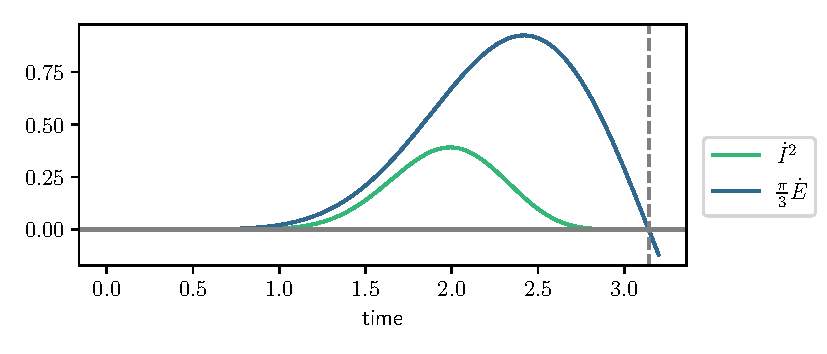
\includegraphics{pendry_propagate_thermal_state_energy_without_ln2_new.pdf}
    \caption{Informationsfluss und Energiefluss für eine Spinkette, bei der
    das erste Qubit in einem gemischten, bzw. thermischen Zustand mit
    inverser Temperatur $\beta = 1/300$ initialisiert wird.
    Der Energiefluss wird hier nur mit $\pi/3$ anstatt mit $\pi/(3\ln^22)$
    multipliziert.}
    \label{fig:pendry-perf-initialstate-thermal}
\end{figure}
Zum Vergleich ist in \cref{fig:pendry-perf-init-spinup-with-and-without-ln2}
der Energiefluss mit und ohne den Faktor $\ln^22$ abgebildet. Es ist deutlich
zu sehen, dass der Faktor notwendig ist, damit die Bound hält.
\begin{figure}[H]
	\centering
	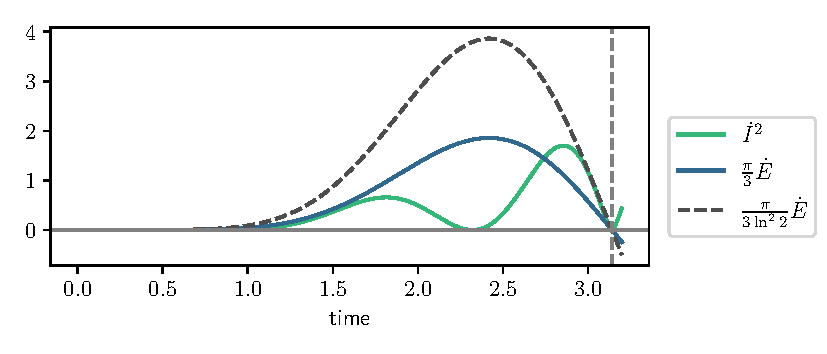
\includegraphics{pendry_propagate_spinup_state_energy_with_and_without_ln2_with=dashed.pdf}
	\caption{Informationsfluss und Energiefluss für eine Spinkette, bei der
	das erste Qubit in einem Spin-Up Zustand, $\rho=\dyad{1}$, initialisiert
	wird. Der Energiefluss ist einmal mit und einmal ohne den Faktor $\ln^22$
	aufgetragen, wobei die gestrichelte Kurve genau die Kurve mit dem Faktor
	darstellt.}
	\label{fig:pendry-perf-init-spinup-with-and-without-ln2}
\end{figure}
\section*{Was bedeutet das?}
Als erstes bedeutet das, dass Pendry für unser System nur unter bestimmten
Voraussetzungen gilt. Für die Verletzung mit den Korrelationen macht das nichts,
da die Korrelationen thermische Zustände erfordern. Da nun aber klar ist, dass da
ein Faktor zu viel ist, ist das Verhalten minimal anders. Der Vorzeichenwechsel
in $\dot{E}$ ist natürlich noch immer gegeben, daher gilt die Verletzung trotzdem.

Eine wesentliche Folgerung ist aber, dass wir für die Systeme ohne korrelierte
Qubits schon eine Verletzung mit einem Spin-up Zustand haben. Das sagt uns, dass
Pendry nicht nur für Systeme mit Korrelationen nicht gilt, sondern vor allem für
Systeme \emph{ohne} Korrelationen, die \emph{nicht} mit einem gemischten Zustand
starten, denen man eine Temperatur zuordnen könnte (also ein thermischer Zustand).
\section*{Die neuen Fragen}
Aus diesen Erkenntnissen lassen sich neue Fragen ableiten, die es (zumindest zum
Teil) zu beantworten gilt. Als erstes die Frage nach einer allgemeineren Bound:
Wie sieht eine Bound aus, die nicht für Spin-up verletzt wird? Der bereits,
irrtümlicherweise, verwendete Faktor $\ln^22$ sorgt dafür, dass die Kette mit
schnellstem perfekten Zustandstransfer die Bound nicht bricht. Ist das schon die
Korrektur, die man braucht, oder kann analytisch noch ein Faktor gefunden werden,
bei dem die Bound genau gesättigt wird? Wäre das überhaupt die Interaktion, bei
der die Bound gerade nicht bricht, oder gibt es noch weitere Spinketten, die nicht
Heisenberg-$XY$ Ketten sind, die schnelleren Zustandstransfer (und damit höheren
Informationsfluss) erlauben?

\printbibliography
\end{document}
